
\chapter{実装}
\label{sec:implementation}

本章では，本研究で使用するVRゲーム環境の実装について説明する．また，本研究では2つの実験を行い，それぞれで使用するオブジェクトを用意し，各タスクに必要な機能を実装した．なお，各実験の具体的な内容や実施方法については，第5章で述べる．

\section{システム構成}
\label{sec:system}

\begin{figure}[htbp]
  \centering
  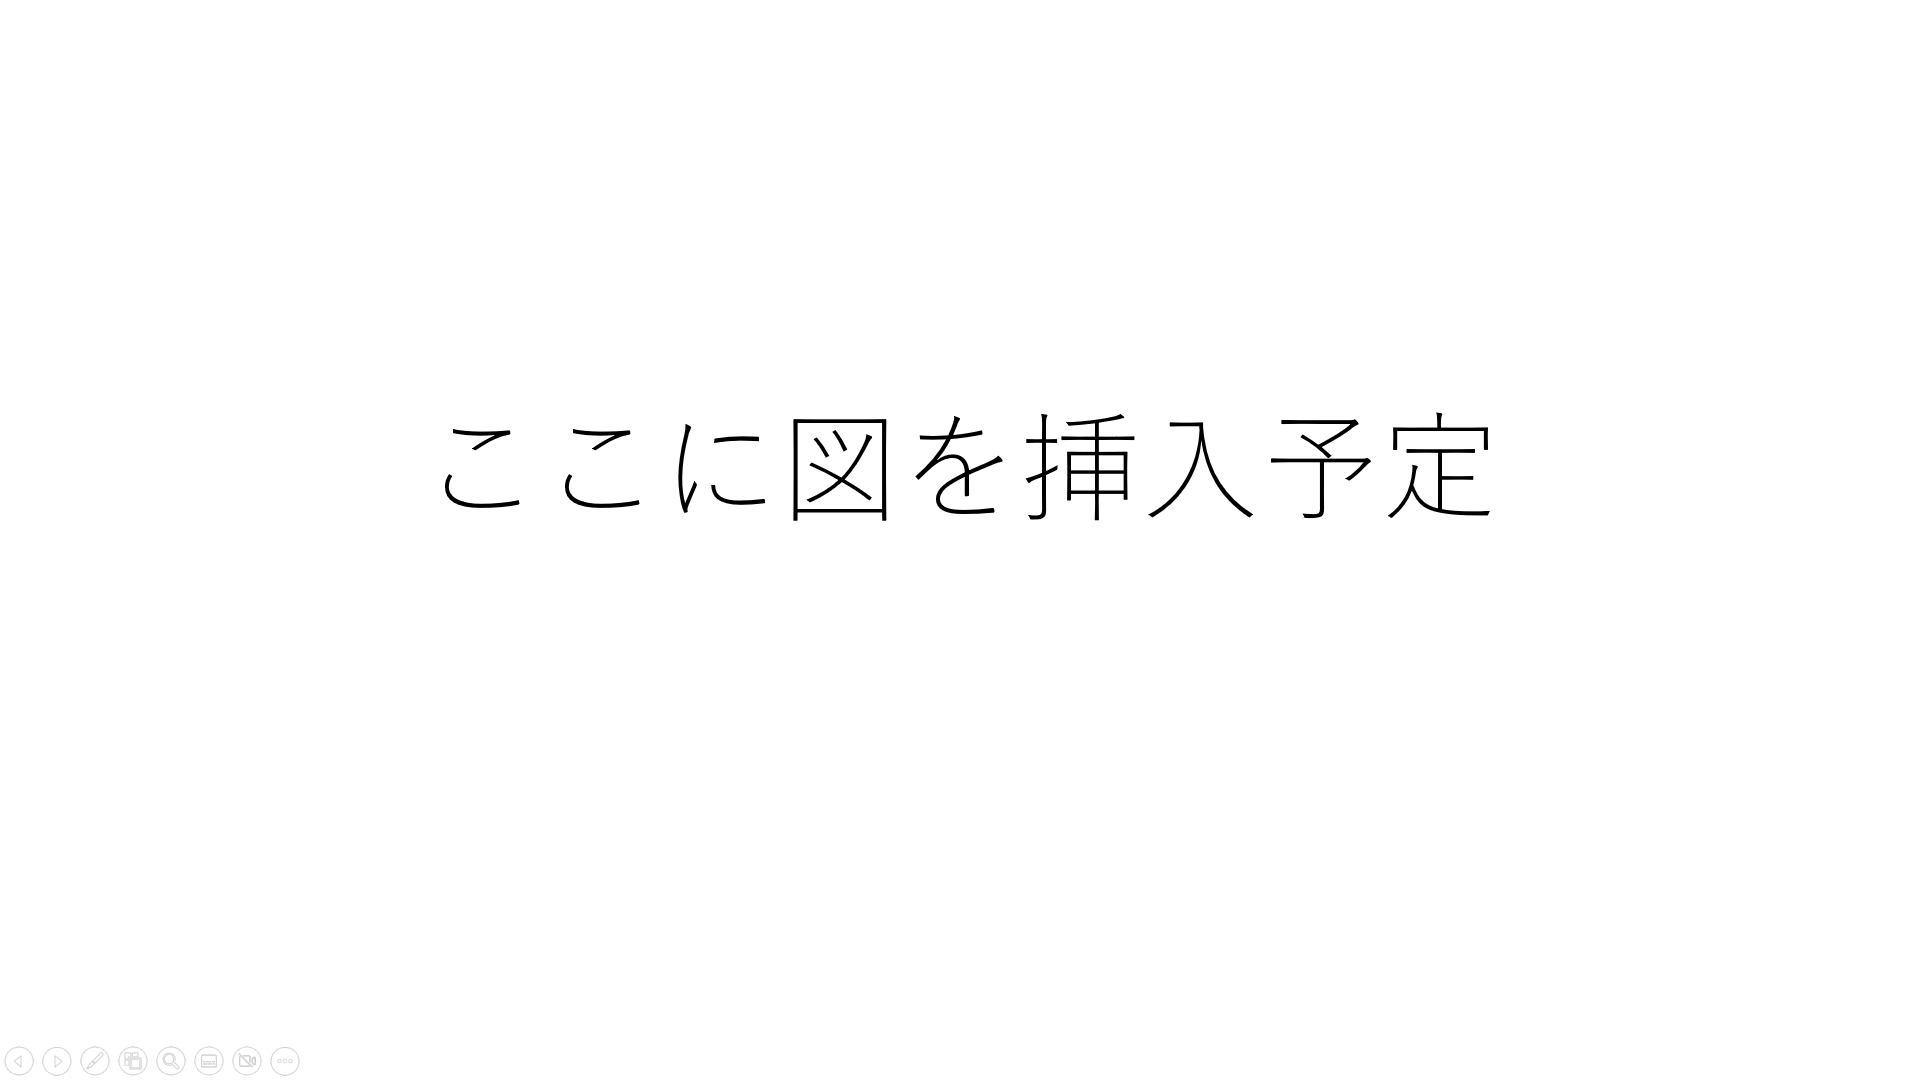
\includegraphics[width=0.8\linewidth]{fig/placeholder.png}
  \caption{システム構成図}
  \label{fig:100}
\end{figure}

本研究では，Unityを用いてVRゲーム環境を構築し，Meta Quest 3を使用する．VR空間には，プレイヤーの視点，ブレス攻撃エフェクト，攻撃対象となるオブジェクトを配置する．プレイヤーは攻撃対象を狙い，ブレス攻撃によって対象を攻撃する．

本研究では，ブレス攻撃エフェクトによる攻撃対象の遮蔽に着目し，4種類の表示条件を比較する．各表示条件の詳細については，第\ref{sec:display}章で述べたとおりである．

\section{ブレス攻撃の実装}
\label{sec:breath_attack}

ブレス攻撃は，UnityのParticle Systemを用いて炎のエフェクトとして表現する．攻撃時には，プレイヤーの視点方向に炎のパーティクルを発生させ，ブレス攻撃を再現する．

攻撃エフェクトの表示方法は，通常表示，半透明表示，奥部透明表示の3種類を実装した．それぞれの表示方法では，パーティクルの透明度や表示状態を変更することで，攻撃対象の見え方を調整する．

攻撃の発生に使用する操作は（仮）とする．攻撃エフェクトの表示時間は（仮）秒とする．また，ブレス攻撃の命中判定には，Particle Systemの衝突判定機能を使用する．

\section{実験用オブジェクトの実装}
\label{sec:objects}

本研究では，二つの実験で使用するオブジェクトとして，的オブジェクトとゴーストオブジェクトを用意した．それぞれのオブジェクトには，各実験で必要となる機能を実装した．

\subsection{的オブジェクト}

\begin{figure}[htbp]
  \centering
  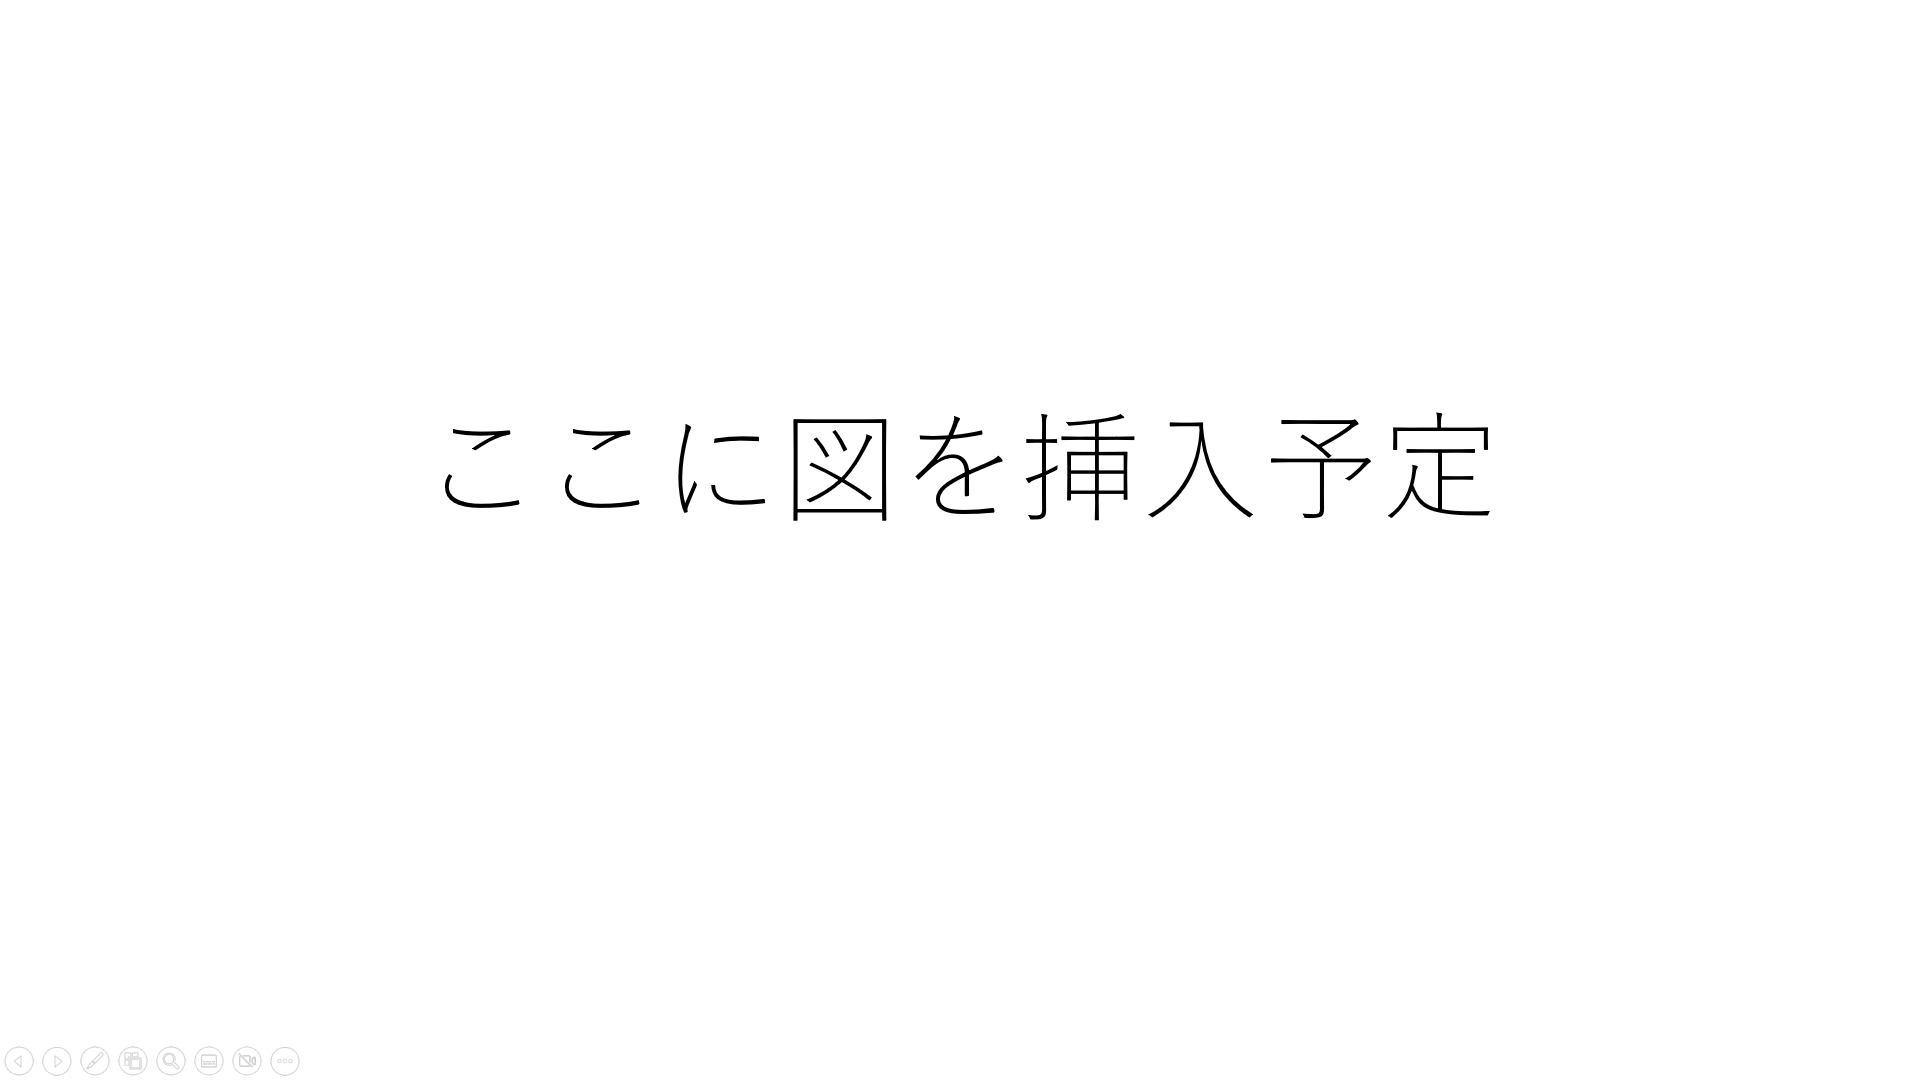
\includegraphics[width=0.8\linewidth]{fig/placeholder.png}
  \caption{的オブジェクト}
  \label{fig:100}
\end{figure}

的オブジェクトは，VR空間内を上下左右のランダムな方向に移動するように設定した．また，移動範囲を制限し，特定の範囲内を移動するようにした．移動速度は（仮），1回の移動時間は（仮），方向転換の間隔は（仮）とした．

さらに，的オブジェクトの中心位置とクロスヘアの位置を取得し，両者の画面上の座標から距離を算出する機能を実装した．算出した距離は一定間隔（仮）でCSVファイルに記録し，実験後の分析に使用する．

\subsection{ゴーストオブジェクト}

ゴーストオブジェクトは，VR空間内をランダムな方向に移動するように設定した．また，移動範囲を制限し，特定の範囲内を移動するようにした．移動速度は（仮），1回の移動時間は（仮），方向転換の間隔は（仮）とした．

ゴーストオブジェクトにはColliderを設定し，ブレス攻撃のパーティクルとの接触を判定できるようにした．パーティクルがゴーストに接触すると，攻撃が命中したと判定し，ゴーストの体力を減少させる．体力が0になるとゴーストは消滅する（消滅処理）．

\begin{figure}[htbp]
  \centering
  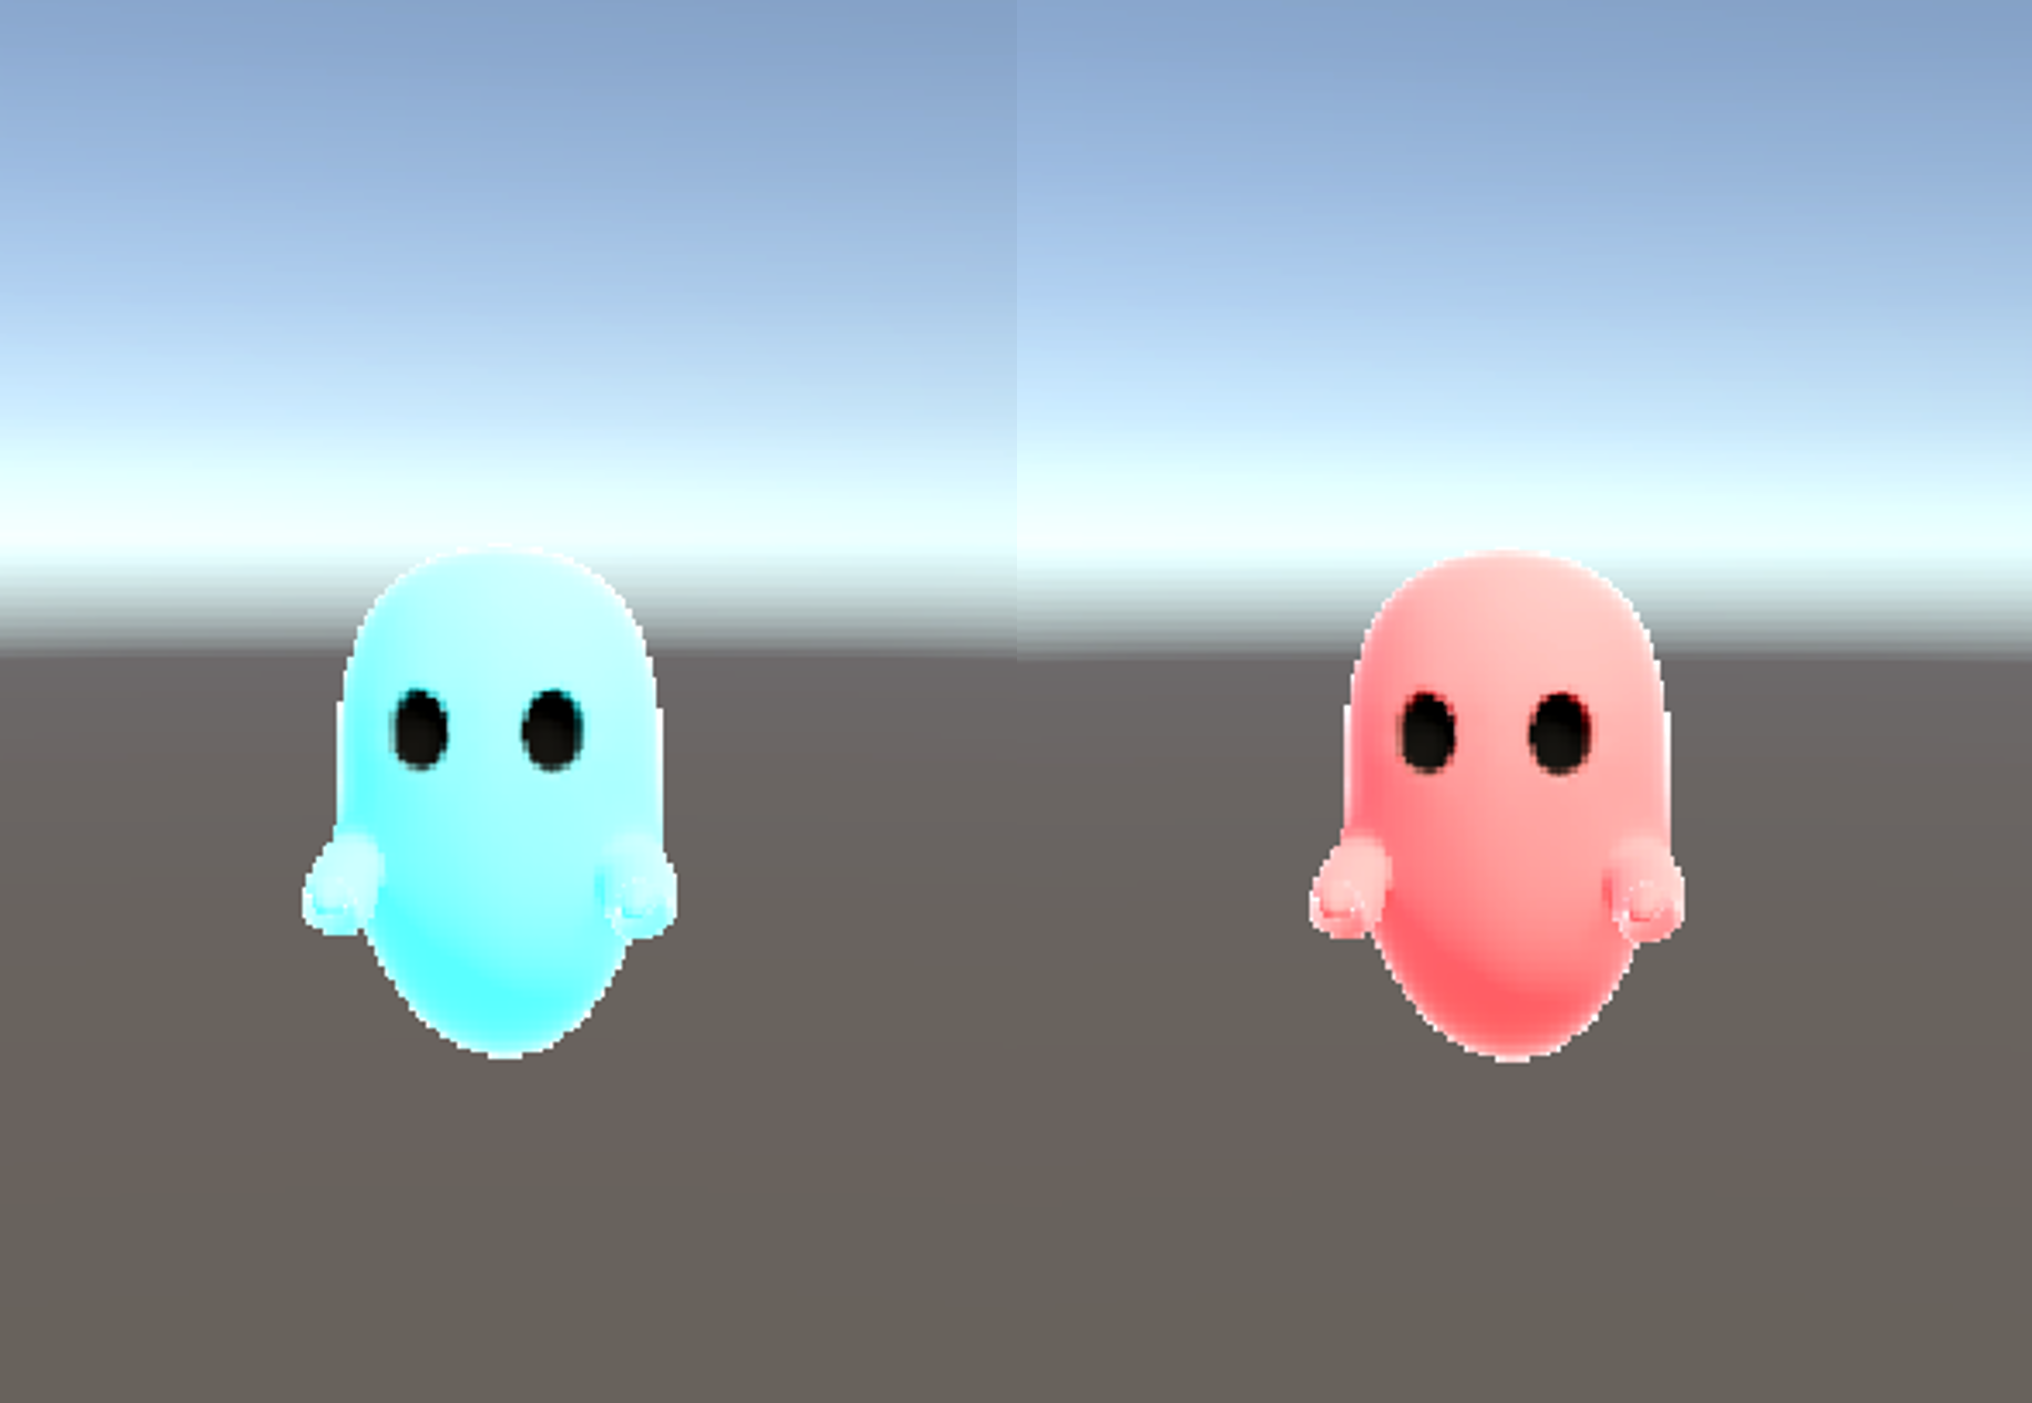
\includegraphics[width=0.8\linewidth]{fig/ghost.png}
  \caption{ゴーストオブジェクトの状態比較(左:攻撃不可能状態,右:攻撃可能状態)}
  \label{fig:4}
\end{figure}


\figref{fig:4}に示すよう,にゴーストには攻撃可能な状態と攻撃不可能な状態を設定した．攻撃可能な状態では青色，攻撃不可能な状態では赤色で表示する．攻撃可能な状態のゴーストに攻撃が命中した場合はスコアを加算し，攻撃不可能な状態のゴーストに攻撃が命中した場合はスコアを減算する（仮）．各状態の継続時間は，攻撃可能な状態を（仮），攻撃不可能な状態を（仮）とした．
